\documentclass[]{article}
\usepackage{lmodern}
\usepackage{amssymb,amsmath}
\usepackage{ifxetex,ifluatex}
\usepackage{fixltx2e} % provides \textsubscript
\ifnum 0\ifxetex 1\fi\ifluatex 1\fi=0 % if pdftex
  \usepackage[T1]{fontenc}
  \usepackage[utf8]{inputenc}
\else % if luatex or xelatex
  \ifxetex
    \usepackage{mathspec}
  \else
    \usepackage{fontspec}
  \fi
  \defaultfontfeatures{Ligatures=TeX,Scale=MatchLowercase}
\fi
% use upquote if available, for straight quotes in verbatim environments
\IfFileExists{upquote.sty}{\usepackage{upquote}}{}
% use microtype if available
\IfFileExists{microtype.sty}{%
\usepackage{microtype}
\UseMicrotypeSet[protrusion]{basicmath} % disable protrusion for tt fonts
}{}
\usepackage[margin=1in]{geometry}
\usepackage{hyperref}
\hypersetup{unicode=true,
            pdftitle={p8105\_hw1\_hs3163},
            pdfauthor={Hao Sun},
            pdfborder={0 0 0},
            breaklinks=true}
\urlstyle{same}  % don't use monospace font for urls
\usepackage{color}
\usepackage{fancyvrb}
\newcommand{\VerbBar}{|}
\newcommand{\VERB}{\Verb[commandchars=\\\{\}]}
\DefineVerbatimEnvironment{Highlighting}{Verbatim}{commandchars=\\\{\}}
% Add ',fontsize=\small' for more characters per line
\usepackage{framed}
\definecolor{shadecolor}{RGB}{248,248,248}
\newenvironment{Shaded}{\begin{snugshade}}{\end{snugshade}}
\newcommand{\AlertTok}[1]{\textcolor[rgb]{0.94,0.16,0.16}{#1}}
\newcommand{\AnnotationTok}[1]{\textcolor[rgb]{0.56,0.35,0.01}{\textbf{\textit{#1}}}}
\newcommand{\AttributeTok}[1]{\textcolor[rgb]{0.77,0.63,0.00}{#1}}
\newcommand{\BaseNTok}[1]{\textcolor[rgb]{0.00,0.00,0.81}{#1}}
\newcommand{\BuiltInTok}[1]{#1}
\newcommand{\CharTok}[1]{\textcolor[rgb]{0.31,0.60,0.02}{#1}}
\newcommand{\CommentTok}[1]{\textcolor[rgb]{0.56,0.35,0.01}{\textit{#1}}}
\newcommand{\CommentVarTok}[1]{\textcolor[rgb]{0.56,0.35,0.01}{\textbf{\textit{#1}}}}
\newcommand{\ConstantTok}[1]{\textcolor[rgb]{0.00,0.00,0.00}{#1}}
\newcommand{\ControlFlowTok}[1]{\textcolor[rgb]{0.13,0.29,0.53}{\textbf{#1}}}
\newcommand{\DataTypeTok}[1]{\textcolor[rgb]{0.13,0.29,0.53}{#1}}
\newcommand{\DecValTok}[1]{\textcolor[rgb]{0.00,0.00,0.81}{#1}}
\newcommand{\DocumentationTok}[1]{\textcolor[rgb]{0.56,0.35,0.01}{\textbf{\textit{#1}}}}
\newcommand{\ErrorTok}[1]{\textcolor[rgb]{0.64,0.00,0.00}{\textbf{#1}}}
\newcommand{\ExtensionTok}[1]{#1}
\newcommand{\FloatTok}[1]{\textcolor[rgb]{0.00,0.00,0.81}{#1}}
\newcommand{\FunctionTok}[1]{\textcolor[rgb]{0.00,0.00,0.00}{#1}}
\newcommand{\ImportTok}[1]{#1}
\newcommand{\InformationTok}[1]{\textcolor[rgb]{0.56,0.35,0.01}{\textbf{\textit{#1}}}}
\newcommand{\KeywordTok}[1]{\textcolor[rgb]{0.13,0.29,0.53}{\textbf{#1}}}
\newcommand{\NormalTok}[1]{#1}
\newcommand{\OperatorTok}[1]{\textcolor[rgb]{0.81,0.36,0.00}{\textbf{#1}}}
\newcommand{\OtherTok}[1]{\textcolor[rgb]{0.56,0.35,0.01}{#1}}
\newcommand{\PreprocessorTok}[1]{\textcolor[rgb]{0.56,0.35,0.01}{\textit{#1}}}
\newcommand{\RegionMarkerTok}[1]{#1}
\newcommand{\SpecialCharTok}[1]{\textcolor[rgb]{0.00,0.00,0.00}{#1}}
\newcommand{\SpecialStringTok}[1]{\textcolor[rgb]{0.31,0.60,0.02}{#1}}
\newcommand{\StringTok}[1]{\textcolor[rgb]{0.31,0.60,0.02}{#1}}
\newcommand{\VariableTok}[1]{\textcolor[rgb]{0.00,0.00,0.00}{#1}}
\newcommand{\VerbatimStringTok}[1]{\textcolor[rgb]{0.31,0.60,0.02}{#1}}
\newcommand{\WarningTok}[1]{\textcolor[rgb]{0.56,0.35,0.01}{\textbf{\textit{#1}}}}
\usepackage{graphicx,grffile}
\makeatletter
\def\maxwidth{\ifdim\Gin@nat@width>\linewidth\linewidth\else\Gin@nat@width\fi}
\def\maxheight{\ifdim\Gin@nat@height>\textheight\textheight\else\Gin@nat@height\fi}
\makeatother
% Scale images if necessary, so that they will not overflow the page
% margins by default, and it is still possible to overwrite the defaults
% using explicit options in \includegraphics[width, height, ...]{}
\setkeys{Gin}{width=\maxwidth,height=\maxheight,keepaspectratio}
\IfFileExists{parskip.sty}{%
\usepackage{parskip}
}{% else
\setlength{\parindent}{0pt}
\setlength{\parskip}{6pt plus 2pt minus 1pt}
}
\setlength{\emergencystretch}{3em}  % prevent overfull lines
\providecommand{\tightlist}{%
  \setlength{\itemsep}{0pt}\setlength{\parskip}{0pt}}
\setcounter{secnumdepth}{0}
% Redefines (sub)paragraphs to behave more like sections
\ifx\paragraph\undefined\else
\let\oldparagraph\paragraph
\renewcommand{\paragraph}[1]{\oldparagraph{#1}\mbox{}}
\fi
\ifx\subparagraph\undefined\else
\let\oldsubparagraph\subparagraph
\renewcommand{\subparagraph}[1]{\oldsubparagraph{#1}\mbox{}}
\fi

%%% Use protect on footnotes to avoid problems with footnotes in titles
\let\rmarkdownfootnote\footnote%
\def\footnote{\protect\rmarkdownfootnote}

%%% Change title format to be more compact
\usepackage{titling}

% Create subtitle command for use in maketitle
\providecommand{\subtitle}[1]{
  \posttitle{
    \begin{center}\large#1\end{center}
    }
}

\setlength{\droptitle}{-2em}

  \title{p8105\_hw1\_hs3163}
    \pretitle{\vspace{\droptitle}\centering\huge}
  \posttitle{\par}
    \author{Hao Sun}
    \preauthor{\centering\large\emph}
  \postauthor{\par}
      \predate{\centering\large\emph}
  \postdate{\par}
    \date{9/14/2019}


\begin{document}
\maketitle

\hypertarget{problem-1}{%
\subsection{Problem 1}\label{problem-1}}

Task 1: Create a data frame comprised of:

\begin{enumerate}
\def\labelenumi{\arabic{enumi}.}
\tightlist
\item
  a random sample of size 8 from a standard Normal distribution
\item
  a logical vector indicating whether elements of the sample are greater
  than 0
\item
  a character vector of length 8
\item
  a factor vector of length 8, with 3 different factor ``levels''
\end{enumerate}

Answer:

\begin{Shaded}
\begin{Highlighting}[]
\CommentTok{#Set the seed for the random Norma distribution}
\KeywordTok{set.seed}\NormalTok{(}\DecValTok{1}\NormalTok{)}
\NormalTok{problem1_df =}\StringTok{ }\KeywordTok{tibble}\NormalTok{(}
  \CommentTok{#the first vector is a random sample of size 8 from a standard Normal distribution}
  \DataTypeTok{vec_random_sample =}\NormalTok{ (}\DataTypeTok{x =} \KeywordTok{rnorm}\NormalTok{(}\DecValTok{8}\NormalTok{) ),}
  \CommentTok{#the second vector is the a character vector of length 8 indexing the sample from normal distribution}
  \DataTypeTok{vec_char =} \KeywordTok{c}\NormalTok{(}\StringTok{"first"}\NormalTok{, }\StringTok{"second"}\NormalTok{, }\StringTok{"third"}\NormalTok{, }\StringTok{"forth"}\NormalTok{,}\StringTok{"fifth"}\NormalTok{,}\StringTok{"sixth"}\NormalTok{,}\StringTok{"seventh"}\NormalTok{,}\StringTok{"eighth"}\NormalTok{),}
  \CommentTok{#the third vector is the logical vector that used to determined whether elements of the sample are greater than 0}
  \DataTypeTok{vec_logical =}\NormalTok{ vec_random_sample }\OperatorTok{>}\StringTok{ }\DecValTok{0}\NormalTok{ ,}
  \CommentTok{#the forth vector is the factor that comprised of three levels.}
  \DataTypeTok{vec_factor =} \KeywordTok{factor}\NormalTok{(}\KeywordTok{c}\NormalTok{(}\StringTok{"low"}\NormalTok{, }\StringTok{"low"}\NormalTok{, }\StringTok{"low"}\NormalTok{, }\StringTok{"middle"}\NormalTok{,}\StringTok{"middle"}\NormalTok{,}\StringTok{"high"}\NormalTok{,}\StringTok{"high"}\NormalTok{,}\StringTok{"high"}\NormalTok{))}
\NormalTok{)}
  
\NormalTok{problem1_df}
\end{Highlighting}
\end{Shaded}

\begin{verbatim}
## # A tibble: 8 x 4
##   vec_random_sample vec_char vec_logical vec_factor
##               <dbl> <chr>    <lgl>       <fct>     
## 1            -0.626 first    FALSE       low       
## 2             0.184 second   TRUE        low       
## 3            -0.836 third    FALSE       low       
## 4             1.60  forth    TRUE        middle    
## 5             0.330 fifth    TRUE        middle    
## 6            -0.820 sixth    FALSE       high      
## 7             0.487 seventh  TRUE        high      
## 8             0.738 eighth   TRUE        high
\end{verbatim}

Task 2: Try to take the mean of each variable in your dataframe. What
works and what doesn't? Answer:

\begin{Shaded}
\begin{Highlighting}[]
\CommentTok{# Find the mean for each vector in the dataset}
\KeywordTok{sapply}\NormalTok{(problem1_df, mean)}
\end{Highlighting}
\end{Shaded}

\begin{verbatim}
## Warning in mean.default(X[[i]], ...): argument is not numeric or logical:
## returning NA

## Warning in mean.default(X[[i]], ...): argument is not numeric or logical:
## returning NA
\end{verbatim}

\begin{verbatim}
## vec_random_sample          vec_char       vec_logical        vec_factor 
##         0.1314544                NA         0.6250000                NA
\end{verbatim}

\begin{Shaded}
\begin{Highlighting}[]
\CommentTok{# Means can be found for numeric or logical vector: vec_random_sample and vec_logical}
\end{Highlighting}
\end{Shaded}

Task 3: In some cases, you can explicitly convert variables from one
type to another. Write a code chunk that applies the as.numeric function
to the logical, character, and factor variables (please show this chunk
but not the output). What happens, and why? Does this help explain what
happens when you try to take the mean?

Answer

\begin{Shaded}
\begin{Highlighting}[]
\CommentTok{#Try to see if the as.numeric function will work on the three vector}
\KeywordTok{sapply}\NormalTok{(}\KeywordTok{select}\NormalTok{(problem1_df,}\DecValTok{2}\OperatorTok{:}\DecValTok{4}\NormalTok{),as.numeric)}

\CommentTok{#It turns out that the as numeric.function works on the logical and factor vector but not the character one. This may be because for the logic vector, one can use number to illustrate the true/false state and for the factor vector, one can use number to indicate what level of the factor it is. However there are no sensible way to do it for the charactor vector. This explain why the charater can not be used to found mean, but did not explian why the factor cannot be used to find mean. }
\end{Highlighting}
\end{Shaded}

Task 4: In a second code chunk:

convert the logical vector to numeric, and multiply the random sample by
the result convert the logical vector to a factor, and multiply the
random sample by the result convert the logical vector to a factor and
then convert the result to numeric, and multiply the random sample by
the result

Answer:

\begin{Shaded}
\begin{Highlighting}[]
\CommentTok{#convert the logical vector to numeric, and multiply the random sample by the result}
\NormalTok{Pb1_Q4_}\DecValTok{1}\NormalTok{<-}\KeywordTok{as.numeric}\NormalTok{(problem1_df}\OperatorTok{$}\NormalTok{vec_logical)}\OperatorTok{*}\StringTok{ }\KeywordTok{pull}\NormalTok{( problem1_df, vec_random_sample)}
\NormalTok{Pb1_Q4_}\DecValTok{1}
\end{Highlighting}
\end{Shaded}

\begin{verbatim}
## [1] 0.0000000 0.1836433 0.0000000 1.5952808 0.3295078 0.0000000 0.4874291
## [8] 0.7383247
\end{verbatim}

\begin{Shaded}
\begin{Highlighting}[]
\CommentTok{#For the false result, the product become zero. For the postive result, the orignin values are retained,}


\CommentTok{#convert the logical vector to a factor, and multiply the random sample by the result}
\KeywordTok{as.factor}\NormalTok{(problem1_df}\OperatorTok{$}\NormalTok{vec_logical)}
\end{Highlighting}
\end{Shaded}

\begin{verbatim}
## [1] FALSE TRUE  FALSE TRUE  TRUE  FALSE TRUE  TRUE 
## Levels: FALSE TRUE
\end{verbatim}

\begin{Shaded}
\begin{Highlighting}[]
\NormalTok{Pb1_Q4_}\DecValTok{2}\NormalTok{<-}\KeywordTok{as.factor}\NormalTok{(problem1_df}\OperatorTok{$}\NormalTok{vec_logical)}\OperatorTok{*}\StringTok{ }\KeywordTok{pull}\NormalTok{( problem1_df, vec_random_sample)}
\end{Highlighting}
\end{Shaded}

\begin{verbatim}
## Warning in Ops.factor(as.factor(problem1_df$vec_logical),
## pull(problem1_df, : '*' not meaningful for factors
\end{verbatim}

\begin{Shaded}
\begin{Highlighting}[]
\NormalTok{Pb1_Q4_}\DecValTok{2}
\end{Highlighting}
\end{Shaded}

\begin{verbatim}
## [1] NA NA NA NA NA NA NA NA
\end{verbatim}

\begin{Shaded}
\begin{Highlighting}[]
\CommentTok{#Since factor is not a numbner, therefore multipilication does not make sense.}

\CommentTok{#convert the logical vector to a factor and then convert the result to numeric, and multiply the random sample by the result}
\NormalTok{Pb1_Q4_}\DecValTok{3}\NormalTok{<-}\KeywordTok{as.numeric}\NormalTok{(}\KeywordTok{as.factor}\NormalTok{(problem1_df}\OperatorTok{$}\NormalTok{vec_logical))}\OperatorTok{*}\StringTok{ }\KeywordTok{pull}\NormalTok{( problem1_df, vec_random_sample)}
\NormalTok{Pb1_Q4_}\DecValTok{3}
\end{Highlighting}
\end{Shaded}

\begin{verbatim}
## [1] -0.6264538  0.3672866 -0.8356286  3.1905616  0.6590155 -0.8204684
## [7]  0.9748581  1.4766494
\end{verbatim}

\begin{Shaded}
\begin{Highlighting}[]
\CommentTok{#Since, when converted to number, the levels of factors will be denoted by 1 and 2 instead of 0 and 1, the result will be different from the first command of this part.}
\end{Highlighting}
\end{Shaded}

\hypertarget{problem-2}{%
\subsection{Problem 2}\label{problem-2}}

Task 1:

This problem focuses the use of inline R code, plotting, and the
behavior of ggplot for variables of different types.

Create a data frame comprised of: x: a random sample of size 500 from a
standard Normal distribution y: a random sample of size 500 from a
standard Normal distribution A logical vector indicating whether x + y
\textgreater{} 1 A numeric vector created by coercing the above logical
vector A factor vector created by coercing the above logical vector
Write a short description of your vector using inline R code, including:
* the size of the dataset (using nrow and ncol) * the mean, median, and
standard deviation of x * the proportion of cases for which x + y
\textgreater{} 1

Answer:

\begin{Shaded}
\begin{Highlighting}[]
\NormalTok{problem2_df =}\StringTok{ }\KeywordTok{tibble}\NormalTok{(}
  \CommentTok{#the first vector is x, a random sample of size 500 from a standard Normal distribution}
  \DataTypeTok{x =}\NormalTok{ (}\DataTypeTok{x =} \KeywordTok{rnorm}\NormalTok{(}\DecValTok{500}\NormalTok{) ),}
 \CommentTok{#the second vector is y, a random sample of size 500 from a standard Normal distribution}
  \DataTypeTok{y =}\NormalTok{ (}\DataTypeTok{y =} \KeywordTok{rnorm}\NormalTok{(}\DecValTok{500}\NormalTok{) ),}
  \CommentTok{#the third vector is the logical vector that used to determined whether x+y >1}
  \DataTypeTok{vec_logical_sum_larger_than_1 =}\NormalTok{ x}\OperatorTok{+}\NormalTok{y }\OperatorTok{>}\StringTok{ }\DecValTok{1}\NormalTok{ ,}
  \CommentTok{#the forth vector is the above logical vector coerced into numeric form}
   \DataTypeTok{pb2_logic_num =} \KeywordTok{as.numeric}\NormalTok{(vec_logical_sum_larger_than_}\DecValTok{1}\NormalTok{),}
 \CommentTok{#the fifth vector is the above logical vector coerced into factor form}
   \DataTypeTok{pb2_logic_factor =} \KeywordTok{as.factor}\NormalTok{(vec_logical_sum_larger_than_}\DecValTok{1}\NormalTok{),}
\NormalTok{ )}

\NormalTok{problem2_df}
\end{Highlighting}
\end{Shaded}

\begin{verbatim}
## # A tibble: 500 x 5
##          x       y vec_logical_sum_larger_t~ pb2_logic_num pb2_logic_factor
##      <dbl>   <dbl> <lgl>                             <dbl> <fct>           
##  1  0.576   1.16   TRUE                                  1 TRUE            
##  2 -0.305  -1.11   FALSE                                 0 FALSE           
##  3  1.51   -2.53   FALSE                                 0 FALSE           
##  4  0.390  -0.936  FALSE                                 0 FALSE           
##  5 -0.621  -0.967  FALSE                                 0 FALSE           
##  6 -2.21    0.0475 FALSE                                 0 FALSE           
##  7  1.12   -0.404  FALSE                                 0 FALSE           
##  8 -0.0449  0.231  FALSE                                 0 FALSE           
##  9 -0.0162 -0.422  FALSE                                 0 FALSE           
## 10  0.944   0.374  TRUE                                  1 TRUE            
## # ... with 490 more rows
\end{verbatim}

the size of the dataset is 5 variable each with the size of 500 The mean
of x is 0.0196843 The median of x is -0.0384371 The standard diviation
of x is 1.0137029 The proportion of cases for which x + y \textgreater{}
1 is 0.252

Task 2: Make a scatterplot of y vs x; color points using the logical
variable (adding color = \ldots{} inside of aes in your ggplot code
should help). Make a second and third scatterplot that color points
using the numeric and factor variables, respectively, and comment on the
color scales.

\begin{Shaded}
\begin{Highlighting}[]
\CommentTok{#scatterplot of y vs x; color points using the logical variable}
\KeywordTok{ggplot}\NormalTok{(problem2_df, }\CommentTok{#Input dataset}
       \KeywordTok{aes}\NormalTok{(}\DataTypeTok{x =}\NormalTok{ x, }\CommentTok{#Define variable that input}
           \DataTypeTok{y=}\NormalTok{y,}
           \DataTypeTok{color =}\NormalTok{ vec_logical_sum_larger_than_}\DecValTok{1}\NormalTok{))}\OperatorTok{+}\KeywordTok{geom_point}\NormalTok{() }\CommentTok{# Define how color are devided and how datapot are arranged.}
\end{Highlighting}
\end{Shaded}

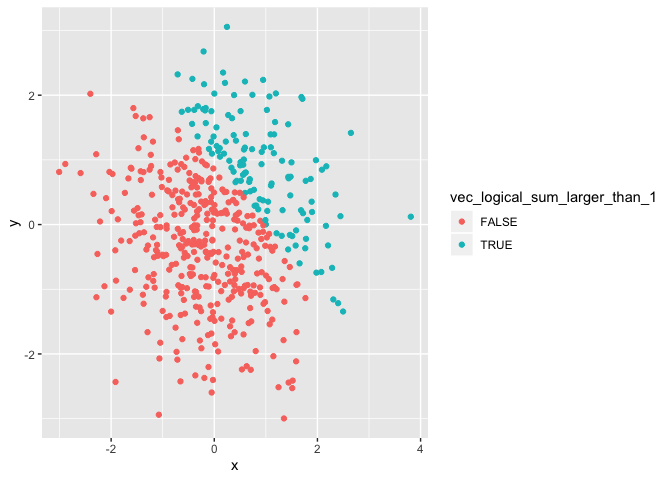
\includegraphics{p8105_hw1_hs3163_files/figure-latex/problem2 task 2 part 1-1.pdf}

\begin{Shaded}
\begin{Highlighting}[]
\CommentTok{#scatterplot of y vs x; color points using the numeric variable}
\KeywordTok{ggplot}\NormalTok{(problem2_df, }\CommentTok{#Input dataset}
       \KeywordTok{aes}\NormalTok{(}\DataTypeTok{x =}\NormalTok{ x, }\CommentTok{#Define variable that input}
           \DataTypeTok{y=}\NormalTok{y,}
           \DataTypeTok{color =}\NormalTok{ pb2_logic_num))}\OperatorTok{+}\KeywordTok{geom_point}\NormalTok{() }\CommentTok{# Define how color are devided and how datapot are arranged.}
\end{Highlighting}
\end{Shaded}

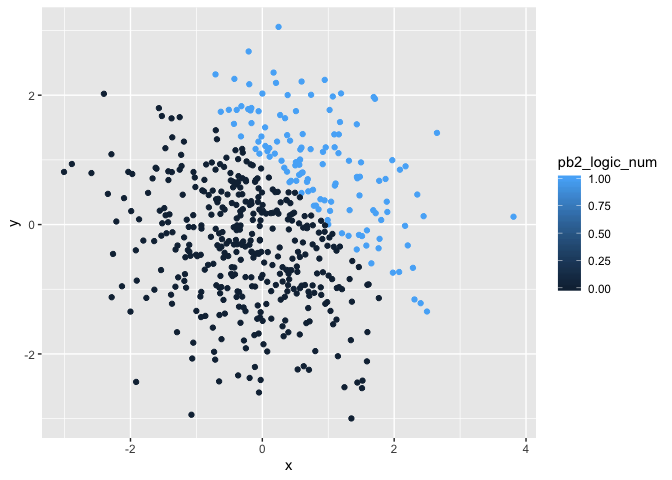
\includegraphics{p8105_hw1_hs3163_files/figure-latex/problem2 task 2 part 2-1.pdf}

\begin{Shaded}
\begin{Highlighting}[]
\CommentTok{#scatterplot of y vs x; color points using the factor variable}
\KeywordTok{ggplot}\NormalTok{(problem2_df, }\CommentTok{#Input dataset}
       \KeywordTok{aes}\NormalTok{(}\DataTypeTok{x =}\NormalTok{ x, }\CommentTok{#Define variable that input}
           \DataTypeTok{y=}\NormalTok{y,}
           \DataTypeTok{color =}\NormalTok{ pb2_logic_factor))}\OperatorTok{+}\KeywordTok{geom_point}\NormalTok{() }\CommentTok{# Define how color are devided and how datapot are arranged.}
\end{Highlighting}
\end{Shaded}

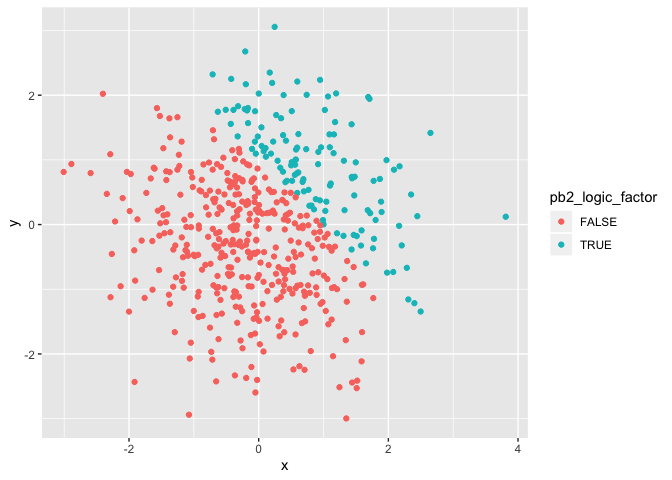
\includegraphics{p8105_hw1_hs3163_files/figure-latex/problem2 task 2 part 3-1.pdf}

Comments on color scale: For the logic and factor vector, the color
scale is binary, while for the numerice vector,the color scale is
continuouse.

Task 3: Export your first scatterplot to your project directory using
ggsave.


\end{document}
